
\documentclass[letterpaper,hide notes,xcolor={table,svgnames},pdftex,10pt]{beamer}
\def\showexamples{t}

\usecolortheme{crane}
\setbeamertemplate{navigation symbols}{}

\usetheme{MyPittsburgh}
\usepackage{hyperref}
\usepackage{graphicx,xspace}
\usepackage[normalem]{ulem}
\usepackage{multicol}
\usepackage{amsmath,amssymb,amsthm,graphicx,xspace}
\newcommand\SF[1]{$\bigstar$\footnote{SF: #1}}

\usepackage[sfdefault,lf]{carlito}
\usepackage[T1]{fontenc}
\usepackage[scaled]{beramono}
\usepackage{tikzpagenodes}
\newcommand{\Rplus}{\protect\hspace{-.1em}\protect\raisebox{.35ex}{\small{\small\textbf{+}}}}
\newcommand{\Cpp}{\mbox{C\Rplus\Rplus}\xspace}

\newcounter{tmpnumSlide}
\newcounter{tmpnumNote}

\newcommand\mnote[1]{%
	\addtocounter{tmpnumSlide}{1}
	\ifdefined\showcues {~\tiny\fbox{\arabic{tmpnumSlide}}}\fi
	\note{\setlength{\parskip}{1ex}\addtocounter{tmpnumNote}{1}\textbf{\Large \arabic{tmpnumNote}:} {#1\par}}}

\newcommand\mmnote[1]{\note{\setlength{\parskip}{1ex}#1\par}}


\newcommand\mquestion[2]{{~\color{red}\fbox{?}}\note{\setlength{\parskip}{1ex}\par{\Large \textbf{?}} #1} \note{\setlength{\parskip}{1ex}\par{\Large \textbf{A}} #2\par}\ifdefined \presentationonly \pause \fi}

\newcommand\blackboard[1]{%
	\ifdefined   \showblackboard
		{#1}
	\else {\begin{center} \fbox{\colorbox{blue!30}{%
						\begin{minipage}{.95\linewidth}%
							\hspace{\stretch{1}} Some space intentionally left blank; done at the blackboard.%
						\end{minipage}}}\end{center}}%
	\fi%
}

\usepackage{listings}
\lstset{%
	keywordstyle=\bfseries,
	aboveskip=15pt,
	belowskip=15pt,
	captionpos=b,
	identifierstyle=\ttfamily,
	frame=lines,
	numbers=left, basicstyle=\scriptsize, numberstyle=\tiny, stepnumber=0, numbersep=2pt}

\usepackage{siunitx}
\newcommand\sius[1]{\num[group-separator = {,}]{#1}\si{\micro\second}}
\newcommand\sims[1]{\num[group-separator = {,}]{#1}\si{\milli\second}}
\newcommand\sins[1]{\num[group-separator = {,}]{#1}\si{\nano\second}}
\sisetup{group-separator = {,}, group-digits = true}

%% -------------------- tikz --------------------
\usepackage{tikz}
\usetikzlibrary{positioning}
\usetikzlibrary{arrows,backgrounds,automata,decorations.shapes,decorations.pathmorphing,decorations.markings,decorations.text}

\tikzstyle{place}=[circle,draw=blue!50,fill=blue!20,thick, inner sep=0pt,minimum size=6mm]
\tikzstyle{transition}=[rectangle,draw=black!50,fill=black!20,thick, inner sep=0pt,minimum size=4mm]

\tikzstyle{block}=[rectangle,draw=black, thick, inner sep=5pt]
\tikzstyle{bullet}=[circle,draw=black, fill=black, thin, inner sep=2pt]

\tikzstyle{pre}=[<-,shorten <=1pt,>=stealth',semithick]
\tikzstyle{post}=[->,shorten >=1pt,>=stealth',semithick]
\tikzstyle{bi}=[<->,shorten >=1pt,shorten <=1pt, >=stealth',semithick]

\tikzstyle{mut}=[-,>=stealth',semithick]

\tikzstyle{treereset}=[dashed,->, shorten >=1pt,>=stealth',thin]

\usepackage{ifmtarg}
\usepackage{xifthen}
\makeatletter
% new counter to now which frame it is within the sequence
\newcounter{multiframecounter}
% initialize buffer for previously used frame title
\gdef\lastframetitle{\textit{undefined}}
% new environment for a multi-frame
\newenvironment{multiframe}[1][]{%
	\ifthenelse{\isempty{#1}}{%
		% if no frame title was set via optional parameter,
		% only increase sequence counter by 1
		\addtocounter{multiframecounter}{1}%
	}{%
		% new frame title has been provided, thus
		% reset sequence counter to 1 and buffer frame title for later use
		\setcounter{multiframecounter}{1}%
		\gdef\lastframetitle{#1}%
	}%
	% start conventional frame environment and
	% automatically set frame title followed by sequence counter
	\begin{frame}%
		\frametitle{\lastframetitle~{\normalfont(\arabic{multiframecounter})}}%
		}{%
	\end{frame}%
}
\makeatother

\makeatletter
\newdimen\tu@tmpa%
\newdimen\ydiffl%
\newdimen\xdiffl%
\newcommand\ydiff[2]{%
	\coordinate (tmpnamea) at (#1);%
	\coordinate (tmpnameb) at (#2);%
	\pgfextracty{\tu@tmpa}{\pgfpointanchor{tmpnamea}{center}}%
	\pgfextracty{\ydiffl}{\pgfpointanchor{tmpnameb}{center}}%
	\advance\ydiffl by -\tu@tmpa%
}
\newcommand\xdiff[2]{%
	\coordinate (tmpnamea) at (#1);%
	\coordinate (tmpnameb) at (#2);%
	\pgfextractx{\tu@tmpa}{\pgfpointanchor{tmpnamea}{center}}%
	\pgfextractx{\xdiffl}{\pgfpointanchor{tmpnameb}{center}}%
	\advance\xdiffl by -\tu@tmpa%
}
\makeatother
\newcommand{\copyrightbox}[3][r]{%
	\begin{tikzpicture}%
		\node[inner sep=0pt,minimum size=2em](ciimage){#2};
		\usefont{OT1}{phv}{n}{n}\fontsize{4}{4}\selectfont
		\ydiff{ciimage.south}{ciimage.north}
		\xdiff{ciimage.west}{ciimage.east}
		\ifthenelse{\equal{#1}{r}}{%
			\node[inner sep=0pt,right=1ex of ciimage.south east,anchor=north west,rotate=90]%
			{\raggedleft\color{black!50}\parbox{\the\ydiffl}{\raggedright{}#3}};%
		}{%
			\ifthenelse{\equal{#1}{l}}{%
				\node[inner sep=0pt,right=1ex of ciimage.south west,anchor=south west,rotate=90]%
				{\raggedleft\color{black!50}\parbox{\the\ydiffl}{\raggedright{}#3}};%
			}{%
				\node[inner sep=0pt,below=1ex of ciimage.south west,anchor=north west]%
				{\raggedleft\color{black!50}\parbox{\the\xdiffl}{\raggedright{}#3}};%
			}
		}
	\end{tikzpicture}
}


%% --------------------

%\usepackage[excludeor]{everyhook}
%\PushPreHook{par}{\setbox0=\lastbox\llap{MUH}}\box0}

%\vspace*{\stretch{1}

%\setbox0=\lastbox \llap{\textbullet\enskip}\box0}

\setlength{\parskip}{\fill}

\newcommand\noskips{\setlength{\parskip}{1ex}}
\newcommand\doskips{\setlength{\parskip}{\fill}}

\newcommand\xx{\par\vspace*{\stretch{1}}\par}
\newcommand\xxs{\par\vspace*{2ex}\par}
\newcommand\tuple[1]{\langle #1 \rangle}
\newcommand\code[1]{{\sf \footnotesize #1}}
\newcommand\ex[1]{\uline{Example:} \ifdefined \presentationonly \pause \fi
	\ifdefined\showexamples#1\xspace\else{\uline{\hspace*{2cm}}}\fi}

\newcommand\ceil[1]{\lceil #1 \rceil}


\AtBeginSection[]
{
	\begin{frame}
		\frametitle{Outline}
		\tableofcontents[currentsection]
	\end{frame}
}



\pgfdeclarelayer{edgelayer}
\pgfdeclarelayer{nodelayer}
\pgfsetlayers{edgelayer,nodelayer,main}

\tikzstyle{none}=[inner sep=0pt]
\tikzstyle{rn}=[circle,fill=Red,draw=Black,line width=0.8 pt]
\tikzstyle{gn}=[circle,fill=Lime,draw=Black,line width=0.8 pt]
\tikzstyle{yn}=[circle,fill=Yellow,draw=Black,line width=0.8 pt]
\tikzstyle{empty}=[circle,fill=White,draw=Black]
\tikzstyle{bw} = [rectangle, draw, fill=blue!20,
text width=4em, text centered, rounded corners, minimum height=2em]

\newcommand{\CcNote}[1]{% longname
	This work is licensed under the \textit{Creative Commons #1 3.0 License}.%
}
\newcommand{\CcImageBy}[1]{%
	\includegraphics[scale=#1]{creative_commons/cc_by_30.pdf}%
}
\newcommand{\CcImageSa}[1]{%
	\includegraphics[scale=#1]{creative_commons/cc_sa_30.pdf}%
}
\newcommand{\CcImageNc}[1]{%
	\includegraphics[scale=#1]{creative_commons/cc_nc_30.pdf}%
}
\newcommand{\CcGroupBySa}[2]{% zoom, gap
	\CcImageBy{#1}\hspace*{#2}\CcImageNc{#1}\hspace*{#2}\CcImageSa{#1}%
}
\newcommand{\CcLongnameByNcSa}{Attribution-NonCommercial-ShareAlike}

\newenvironment{changemargin}[1]{% 
	\begin{list}{}{% 
		\setlength{\topsep}{0pt}% 
		\setlength{\leftmargin}{#1}% 
		\setlength{\rightmargin}{1em}
		\setlength{\listparindent}{\parindent}% 
		\setlength{\itemindent}{\parindent}% 
		      \setlength{\parsep}{\parskip}% 
		      }% 
		\item[]}{\end{list}}



\newcounter{pf}

\title{Lecture 11 --- Memory-Mapped I/O}

\author{Jeff Zarnett \& Mike Cooper-Stachowsky \\ \small \texttt{jzarnett@uwaterloo.ca, mstachowsky@uwaterloo.ca}}
\institute{Department of Electrical and Computer Engineering \\
  University of Waterloo}
\date{\today}

\begin{document}

\begin{frame}
  \titlepage

 \end{frame}


\begin{frame}
\frametitle{Take Me There}

Memory-mapped I/O -- to communicate with a HW device, an area that looks like main memory really represents the HW device.

This simplifies some operations!

Kind of like how UNIX treats everything as a file...

\end{frame}

\begin{frame}
\frametitle{Port Mapped}

This contrasts with the older-style \alert{port-mapped} I/O

There are different CPU instructions and separate registers used to communicate with the device. 

\begin{center}
	
\includegraphics[width=0.4\textwidth]{images/translator.jpg}
\end{center}

It's not that this does not work, but it's just more difficult to work with.

\end{frame}


\begin{frame}
\frametitle{I/O or Control}

Maybe a better name for this is ``Memory Mapped Control''.

The device is controlled via setting some voltages (1s, 0s) on the chip.

If we map those to memory locations, we know how to read write the 1s and 0s to the device just as if it were memory.

\end{frame}


\begin{frame}
\frametitle{Peripheral}

Hardware devices outside the CPU and memory are sometimes referred to as peripheral devices.

A peripheral is an often optional circuit that interfaces with the CPU.

Examples: UART, I2C, GPIO...

\end{frame}


\begin{frame}
\frametitle{Circuit Problem}

The physical connectors that link one device to the motherboard are called pins.

\begin{center}
	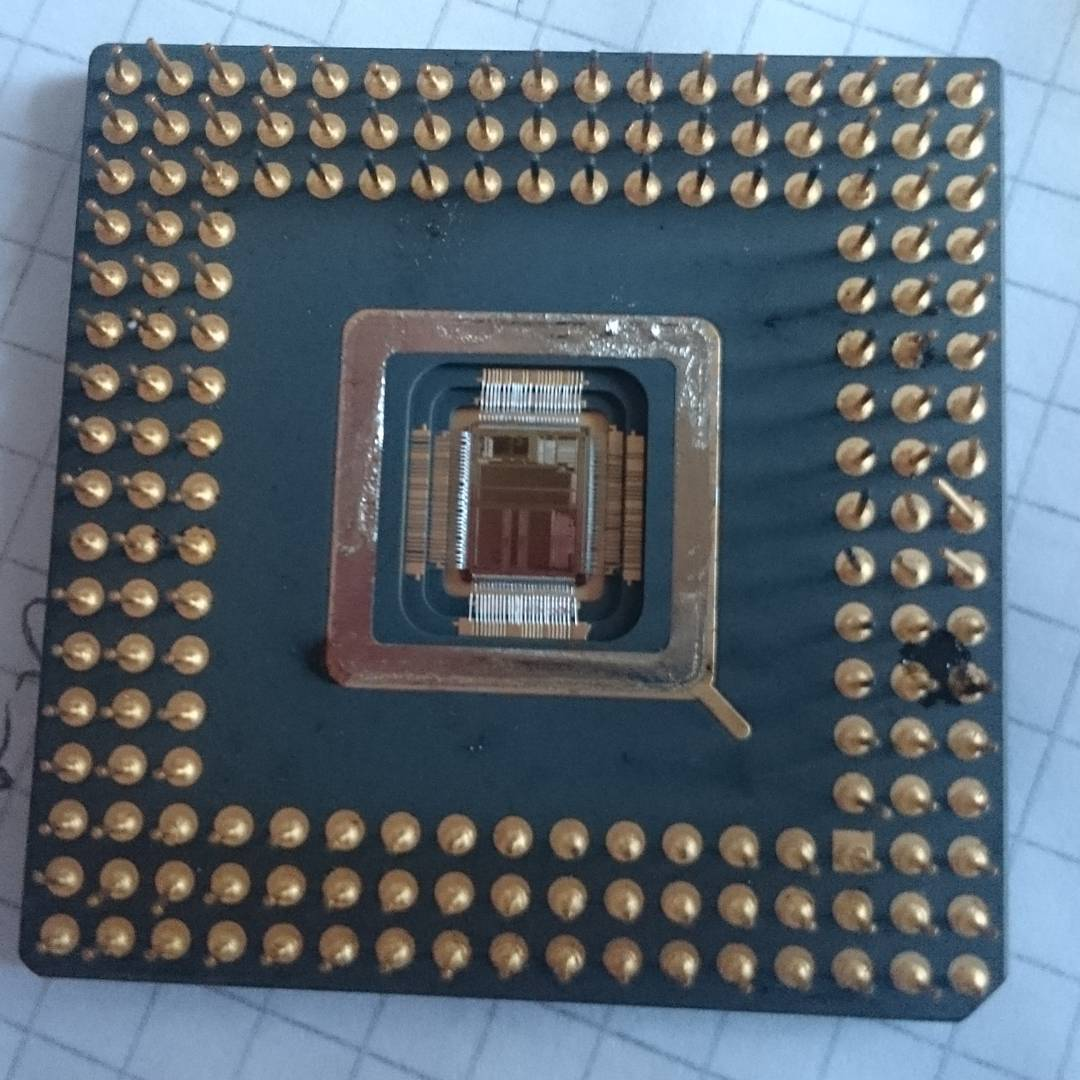
\includegraphics[width=0.5\textwidth]{images/686-cpu.jpg}
\end{center}


\end{frame}


\begin{frame}
\frametitle{Pin Management}

The chip only has a fixed number; some pins do multiple things...
\quad But only ever one at a time.

This implies a need to configure things!

Alright, but let's think about how to control a device...\\
\quad We need to send data out to those pins.

\end{frame}


\begin{frame}
\frametitle{Okay, but where are they?}

The data sheet for the device will tell you where the registers are.

One option: absolute address (which is nice).

Other option: base and offset locations.

Why base and offset? Support multiple devices.


\end{frame}


\begin{frame}
\frametitle{Register Types}

\textbf{Configuration}: Set up the device.

\textbf{Data}: Read/Write data locations.

\textbf{Control}: Tell the device what to do!

\end{frame}


\begin{frame}
\frametitle{STM Did What?}

The chip has multiple GPIO ports so it's base + offset.

Base locations are given in the memory map; offset in GPIO's documentation.

Addresses are the byte address, but registers are often 32 bits.

\end{frame}




\begin{frame}
\frametitle{Global Enable}


\begin{center}
	
\includegraphics[width=0.4\textwidth]{images/plugin.png}
\end{center}

Some chips require global settings or signals to be sent to them.

Example: anything that uses the clock signal needs it sent to it!

\end{frame}


\begin{frame}
\frametitle{Let's talk RCC}

\alert{RCC}: Reset and Clock Control

These are registers used to manage power.

If we don't need a peripheral, don't send it the clock signal!

If it doesn't get the clock signal, it does nothing and saves power.


\end{frame}


\begin{frame}
\frametitle{RCC Base Address}

\begin{center}
	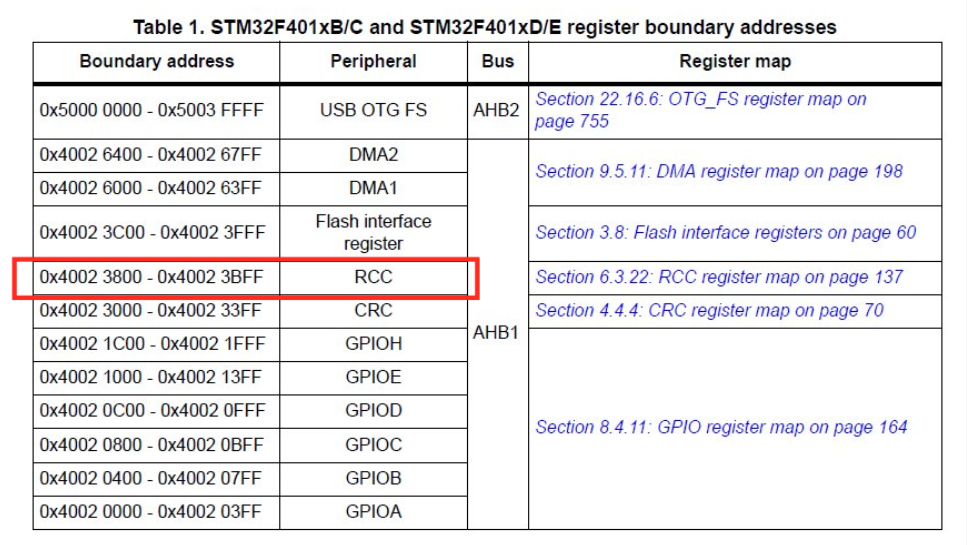
\includegraphics[width=0.95\textwidth]{images/rcc-base.png}
\end{center}


\end{frame}


\begin{frame}
\frametitle{\texttt{RCC\_AHB1ENR}}

What's \texttt{RCC\_AHB1ENR}? AHB is ``Advanced High-Speed Bus''

This is a bus that controls some peripherals including GPIO.

This register controls whether the input has a clock signal. 

Offset is \texttt{0x30}.

\begin{center}
	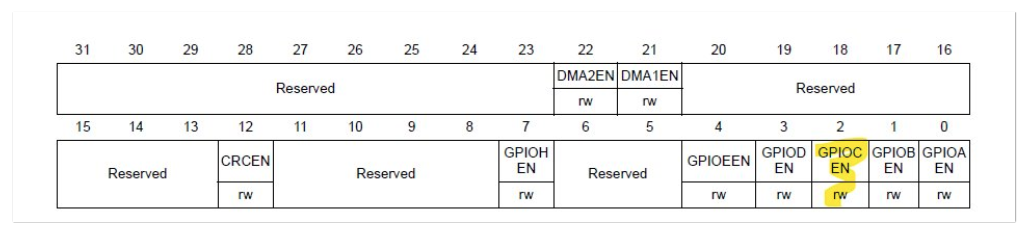
\includegraphics[width=\textwidth]{images/rcc-ahb.png}
\end{center}

\end{frame}


\begin{frame}
\frametitle{GPIO?!}

What is GPIO then? General-Purpose Input/Output

The GPIO system is controlling the voltages on the pins.
 
What's it good for?

\end{frame}


\begin{frame}
\frametitle{GPIO Ideas}

Slow digital input -- signal detection, not data transfer.

Slow digital output -- turning things on/off, not data transfer.

Analog input (ADC)

Other fun stuff if needed: ``Alternate Functions''.

\end{frame}


\begin{frame}
\frametitle{GPIO Organization}

Pins are organized into \alert{ports} of up to 16 pins.

Ports are \texttt{PA*} through \texttt{PC*} on our chip.

Each port is controlled via registers labelled \texttt{GPIOx...}

\begin{center}
	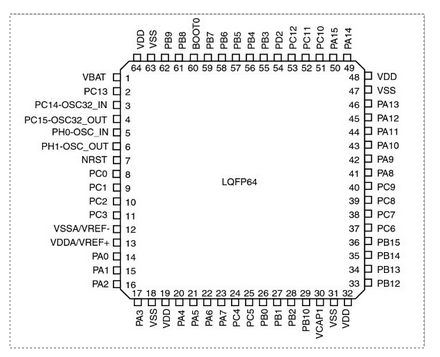
\includegraphics[width=0.5\textwidth]{images/gpio-chip.png}
\end{center}

\end{frame}


\begin{frame}
\frametitle{GPIO Base Addresses}

\begin{center}
	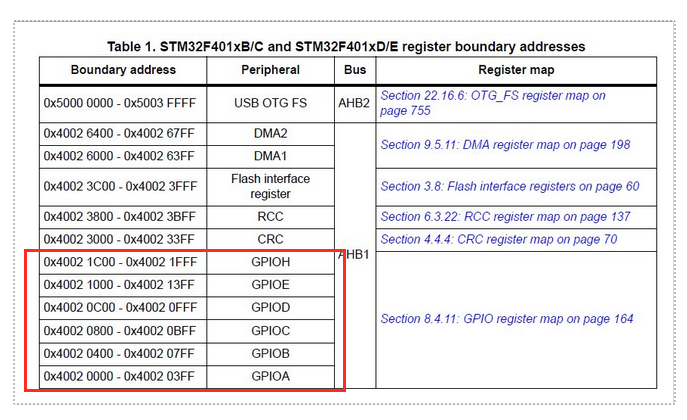
\includegraphics[width=\textwidth]{images/gpio-base.png}
\end{center}


\end{frame}


\begin{frame}
\frametitle{GPIO Configuration Registers}

\texttt{GPIOx\_MODER}: I/O direction, analog or alternate function

\texttt{GPIOx\_OTYPER}: Output type (push/pull, open-drain)

\texttt{GPIOx\_OSPEEDR}: Speed for update/read data

\texttt{GPIOx\_PUPDR}: Pullup/pulldown resistor enable, regardless of direction

\end{frame}


\begin{frame}
\frametitle{What are the Modes?}

The mode register is 32 bits with offset of \texttt{0x00}. 

4 modes are available (2 bits per pin).

\begin{center}
	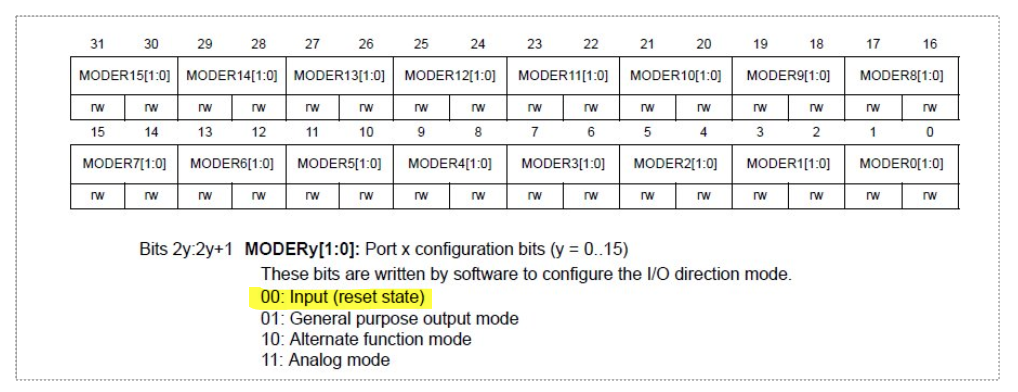
\includegraphics[width=\textwidth]{images/gpio-moder.png}
\end{center}

\end{frame}


\begin{frame}
\frametitle{Alternate Functions}

Alternate Functions just mean using one of the manufacturer-specific functions.

To use them, set the \texttt{GPIOx\_AF} registers.

16 AFs per pin are allowed; 4 bits per pin.

Two AF registers per port: LOW and HIGH.

We won't worry about these until we must.

\end{frame}


\begin{frame}
\frametitle{Other Registers}

Other registers exist but we can usually just use them in their reset state.

If you need something, you can always look up what you need it to be.

\begin{center}
	
\includegraphics[width=0.4\textwidth]{images/halfthebattle.jpg}
\end{center}


\end{frame}

\begin{frame}
\frametitle{GPIO Input/Output Registers}

\texttt{GPIOx\_ODR}: Output data register, must be OUTPUT mode.\\
\quad This is the data! If bit \texttt{j} is 1, the pin \texttt{j} is HIGH.\\
\quad Read-write.

\texttt{GPIOx\_IDR}: Input data register, must be INPUT mode.\\
\quad Stores data read by the pins, read-only.


\end{frame}



\begin{frame}
\frametitle{\texttt{GPIOx\_ODR}}

Offset is \texttt{0x14}.

Only bits 0 to 15 are valid (pins 0 to 15); others are reserved (cannot use).

Used only in output mode -- writing in other modes does nothing.

Write 1 or 0 to write HIGH or LOW on a given pin.\\
\quad Can read back to know what was written.

\end{frame}


\begin{frame}
\frametitle{\texttt{GPIOx\_IDR}}

Offset is \texttt{0x10}.

Only bits 0 to 15 are valid (pins 0 to 15); others are reserved (cannot use).

Used only in input mode -- reads in other modes return garbage.

Read-only.

\end{frame}


\begin{frame}
\frametitle{Basic GPIO Driver}

Very basic GPIO driver: Read PC 13 (user button 1), write to PA5 (LED 2, green).

General plan:

\begin{itemize}
	\item Define registers and offsets needed
	\item Create setup functions
	\item Create read functions for inputs
	\item Create write functions for outputs
\end{itemize}

\begin{center}
	
\includegraphics[width=0.3\textwidth]{images/comingtogether.jpg}
\end{center}

\end{frame}


\begin{frame}[fragile]
\frametitle{Define Statements}

\begin{lstlisting}[language=C]
#include <stdint.h>
#include <stdbool.h>

#define _IDR_OFFSET 0x10
#define _ODR_OFFSET 0x14

#define _RCC_BASE 0x40023800
#define _RCC_GPIO_EN_OFFSET 0x30
#define _GPUI_CLOCK_EN *(uint32_t*) (_RCC_BASE + _RCC_GPIO_EN_OFFSET)

#define _GPIOC_BASE 0x40020800
#define _GPIOC_MODER *(uint32_t*) (_GPIOC_BASE)
#define _GPIOC_IDR *(uint16_t) (_GPIOC_BASE + _IDR_OFFSET)

#define _GPIOA_BASE 0x40020000
#define _GPIOC_MODER *(uint32_t*) (_GPIOA_BASE)
#define _GPIOC_ODR *(uint16_t) (_GPIOA_BASE + _ODR_OFFSET)
\end{lstlisting}


\end{frame}


\begin{frame}[fragile]
\frametitle{Setup}

\begin{lstlisting}[language=C]
void setGPIOCInput() {
  // Enable clock
  _GPIO_CLOCK_EN |= 1<<2;
  _GPIOC_MODER &= ~(0x3 << 26);
}

void setGPIOAOutput() {
  // Clear it first
  _GPIOA_MODER &= ~(0x3 << 10);
  _GPIOA_MODER |= 1 << 10;
}
\end{lstlisting}

\end{frame}

\begin{frame}[fragile]
\frametitle{Access}

\begin{lstlisting}[language=C]
int readGPIOC() {
  return (_GPIOC_IDR & 1<<13) >> 13;
}

void writeGPIOA(bool in) {
  if (in) {
    _GPIOA_ODR |= 1<<5;
  } else {
    _GPIOA_ODR &= ~(1<<5);
  }
}
\end{lstlisting}

\end{frame}

\begin{frame}[fragile]
\frametitle{User}

\begin{lstlisting}[language=C]
while( 1 ) {
  writeGPIOA( !readGPIOC() ); 
}
\end{lstlisting}

It's simple, but it does work!

We can take this template and use it to interact with other I/O devices.

But before we leave the topic, maybe you had a different idea of what memory-mapped I/O is...

\end{frame}



\begin{frame}
	\frametitle{Consult the Map}

	\begin{center}
		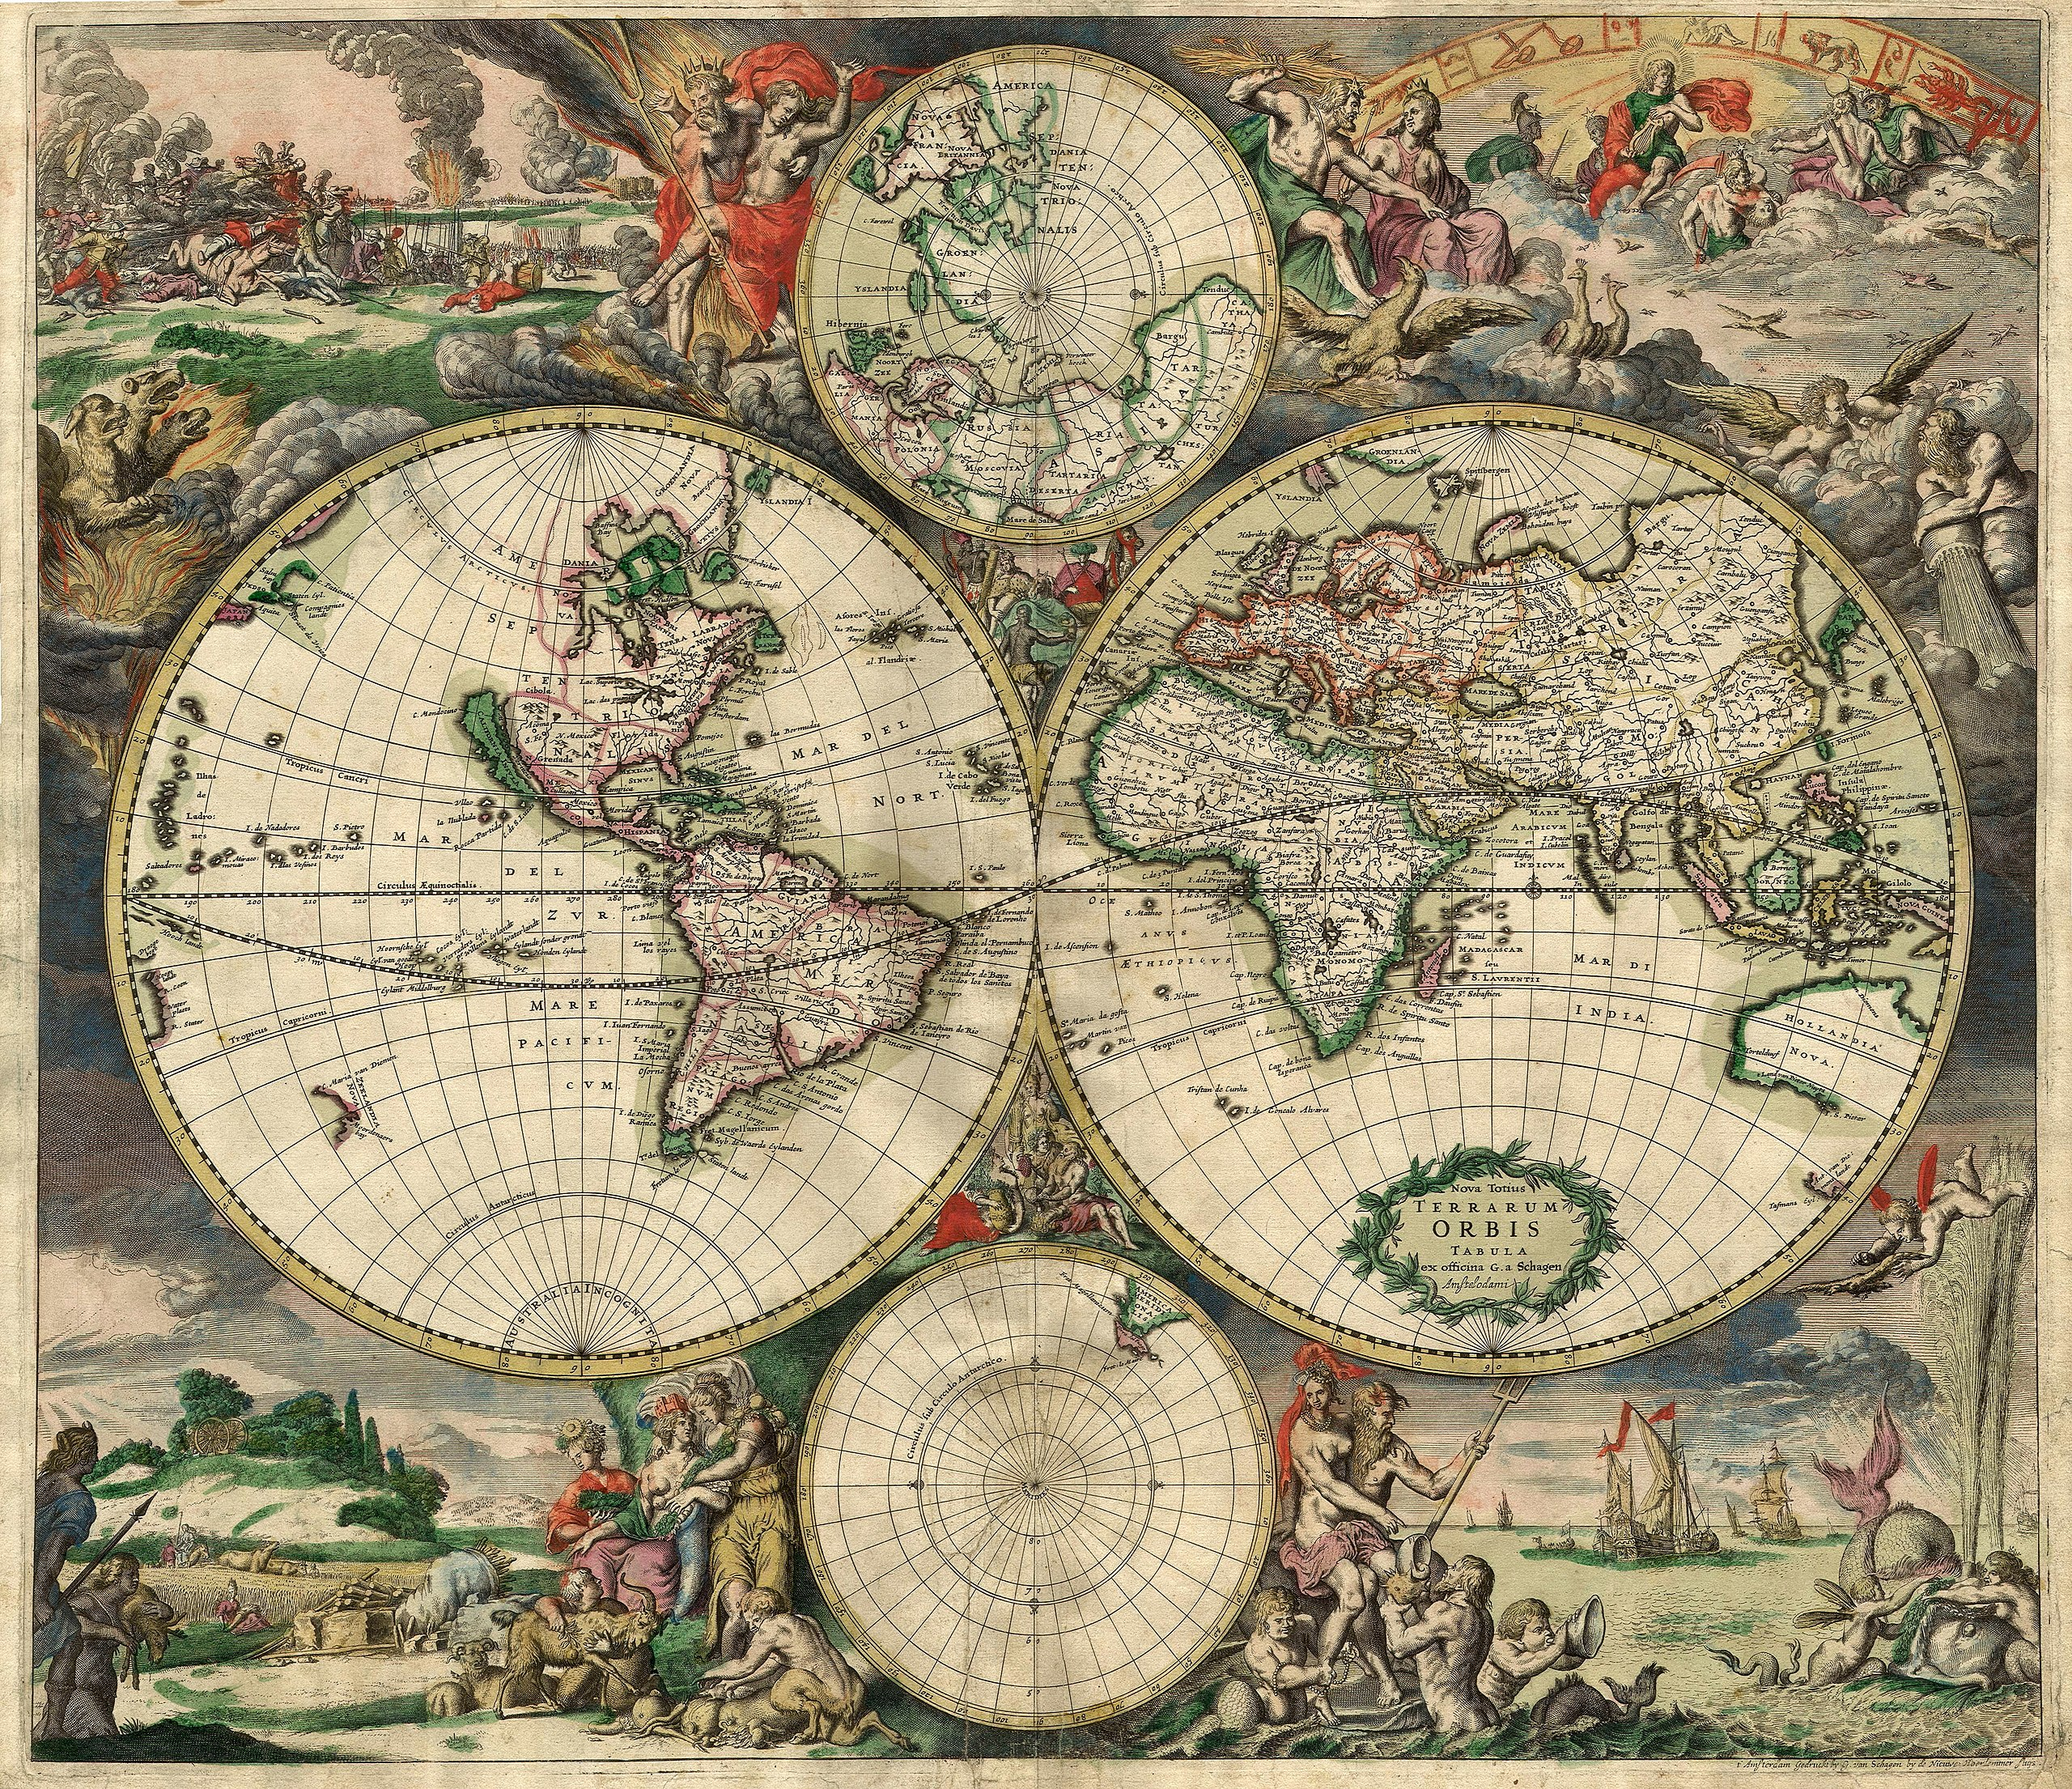
\includegraphics[width=0.8\textwidth]{images/worldmap.jpg}
	\end{center}


\end{frame}


\begin{frame}
	\frametitle{Altenative: \texttt{mmap()}}

	An alternative use for memory-mapping in UNIX involves the use of \texttt{mmap()}, a function nominally used to map a file into memory.

	Then, interact with the file just like memory!

\end{frame}


\begin{frame}[fragile]
	\frametitle{Mapping}
	\begin{lstlisting}[language=C]
void* mmap( void* address, size_t length, int protection, int flag,
   int fd, off_t offset );
\end{lstlisting}

	\texttt{address}: where you want the mapped region to go; use \texttt{NULL}.

	\texttt{length}: how many bytes to map.

	\texttt{protection}: rules for how memory can be used.

	\texttt{flag}: mode for mapping.

	\texttt{fd}: file descriptor of the file to map.

	\texttt{offset}: how far from the start of the file mapping begins.

\end{frame}


\begin{frame}
	\frametitle{Protection Flags}

	Valid values are \texttt{PROT\_NONE}, \texttt{PROT\_READ}, \texttt{PROT\_WRITE}, and \texttt{PROT\_EXECUTE}.

	They can be combined with the bitwise OR operator.

	Whatever flags you choose have to be consistent with how the file was opened with \texttt{open}.

\end{frame}


\begin{frame}
	\frametitle{\texttt{PROT\_NONE}}

	\begin{center}
		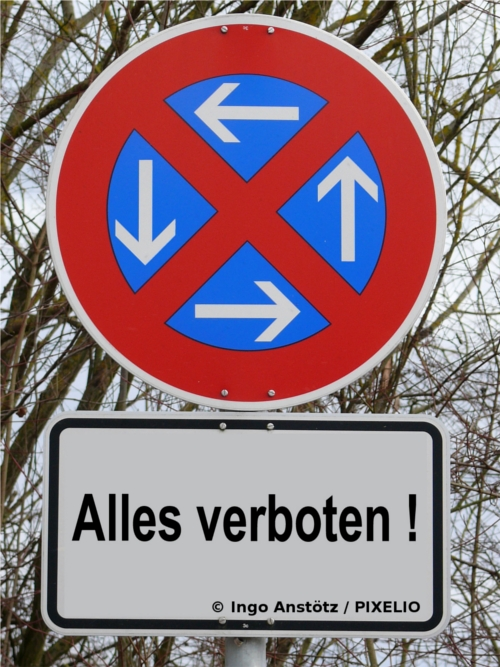
\includegraphics[width=0.45\textwidth]{images/AllesVerboten.jpg}
	\end{center}

	What's the point of \texttt{PROT\_NONE}, if all things are forbidden?

\end{frame}


\begin{frame}
	\frametitle{Flags}
	Flags can be one of two options: \texttt{MAP\_PRIVATE} or \texttt{MAP\_SHARED}.

	Private: modifications are not visible to other processes mapping the same file and not written out to the underlying file.

	Shared: modifications are visible to other processes and written out to the file... but maybe not instantly.

\end{frame}


\begin{frame}
	\frametitle{Memory Mapped File}

	\begin{center}
		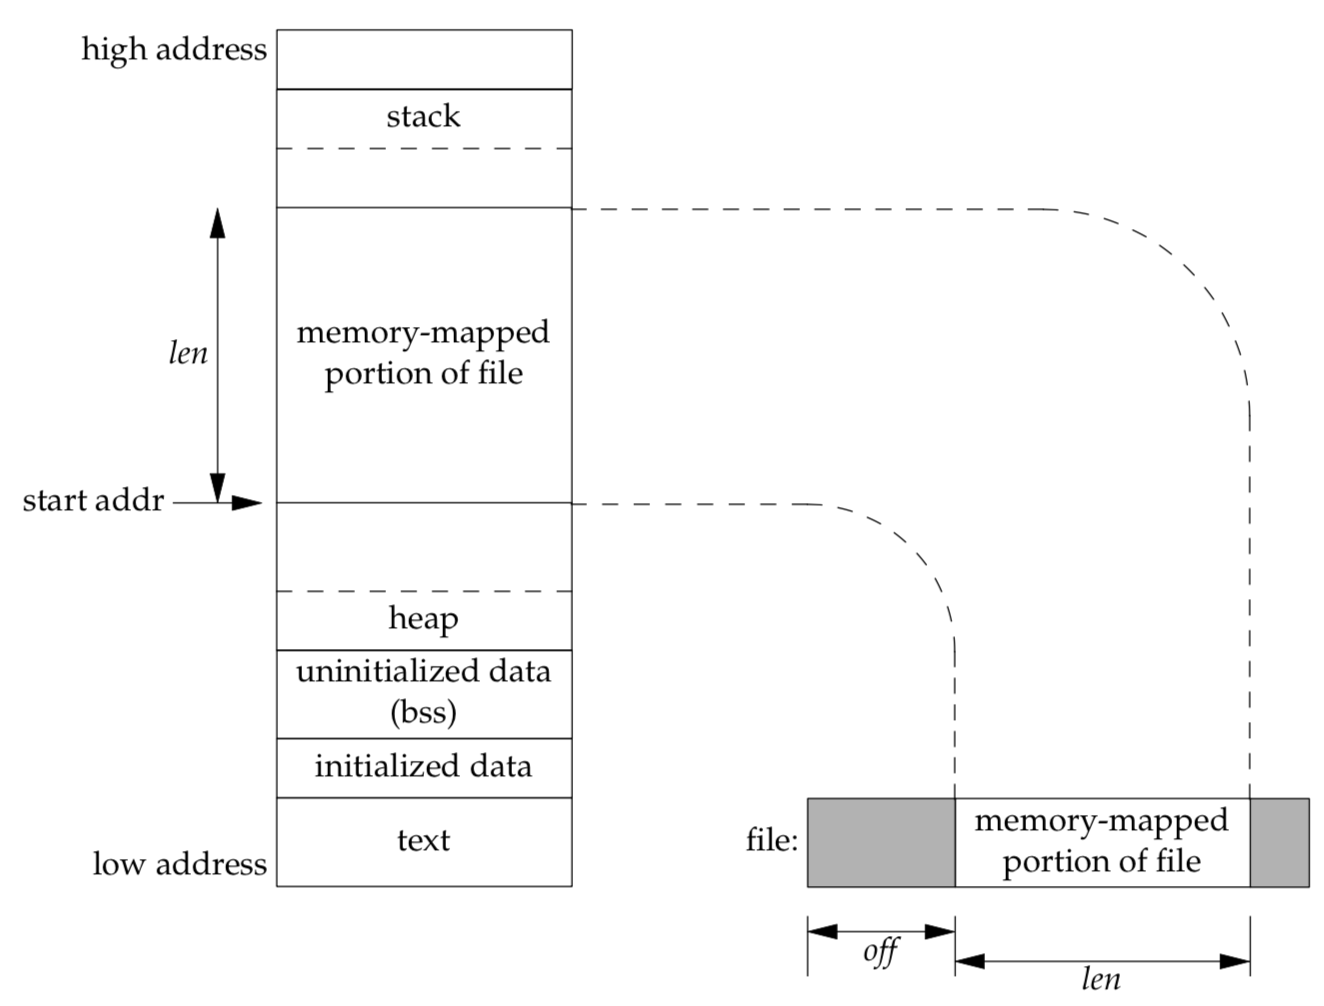
\includegraphics[width=0.9\textwidth]{images/memory-mapped-file.png}
	\end{center}

\end{frame}


\begin{frame}[fragile]
	\frametitle{Protection}

	If we wish to change the protection rules for a section, we use \texttt{mprotect}.

	\begin{lstlisting}[language=C]
int mprotect( void* address, size_t length, int prot );
\end{lstlisting}

	\texttt{address}: the memory to modify protection of.

	\texttt{length}: the size of said memory.

	\texttt{prot}: the new protection rules.

\end{frame}


\begin{frame}[fragile]
	\frametitle{Synchronize}

	\begin{center}
		
\includegraphics[width=0.3\textwidth]{images/sync-icon.png}
	\end{center}

	\begin{lstlisting}[language=C]
int msync( void* address, size_t length, int flags );
\end{lstlisting}

	\texttt{address}: the memory to synchronize.

	\texttt{length}: how many bytes to synchronize.

	\texttt{flags}: mode for synchronization; use \texttt{MS\_SYNC} (blocking).

\end{frame}


\begin{frame}[fragile]
	\frametitle{Unmap}

	\begin{lstlisting}[language=C]
int munmap( void* address, size_t length );
\end{lstlisting}

	\texttt{address}: the memory to unmap.

	\texttt{length}: how many bytes to unmap.

	A segment would be unmapped automatically when a process exits, but as always it is polite to unmap it as soon as you know that you are done with it.

\end{frame}


\begin{frame}[fragile]
	\frametitle{Memory Mapping Example}

	\begin{lstlisting}[language=C]
#define _XOPEN_SOURCE
#include <stdio.h>
#include <stdlib.h>
#include <sys/shm.h>
#include <string.h>
#include <unistd.h>
#include <sys/wait.h>
#include <sys/stat.h>
#include <fcntl.h>
#include <sys/mman.h>

int main( int argc, char** argv ) { 

    int fd = open( "example.txt", O_RDWR );
    
    struct stat st; 
    stat( "example.txt", &st );
    ssize_t size = st.st_size;
    void* mapped = mmap( NULL, size, PROT_READ | PROT_WRITE, MAP_SHARED, fd, 0 );  
\end{lstlisting}
\end{frame}

\begin{frame}[fragile]
	\frametitle{Memory Mapping Example}

	\begin{lstlisting}[language=C]
    int pid = fork();
    if ( pid > 0 ) { /* Parent */
        waitpid( pid, NULL, 0 );
        printf("The new content of the file is: %s.\n", (char*) mapped);
        munmap( mapped, size );
    } else if ( pid == 0 ) { /* Child */
       memset( mapped, 0, size ); /* Erase what's there */
       sprintf( mapped, "It is now Overwritten");
       /* Ensure data is synchronized */
       msync( mapped, size, MS_SYNC );
       munmap( mapped, size );
    }
    close( fd );
    return 0;
}
\end{lstlisting}

\end{frame}

\begin{frame}
	\frametitle{The Example is... Flawed}

	The example works acceptably in the sense that we successfully overwrite the data with the new data and the parent process sees the change.

	But things get weird if we tried to write fewer bytes than the original message.

	In general, the mapped area size cannot change.

	Linux has \texttt{mremap} but this is not portable...

\end{frame}

\begin{frame}
\frametitle{Memory-Mapped Files}

How does it work, though?

Basic premise: disk blocks mapped to main memory.

First access is a page fault; subsequent accesses are reads/writes.

\end{frame}




\end{document}

